\documentclass[a4paper]{article}  
\usepackage{ctex}
\usepackage{graphicx}
\usepackage{geometry}
\usepackage{hyperref}
\usepackage{fancyhdr}  
\hypersetup{
colorlinks=true,
linkcolor=black
}
\geometry{left=2.5cm,right=2.5cm,top=2.5cm,bottom=2.5cm}

\pagestyle{fancy}                 
% 设置页眉页脚风格为 fancyhdr 提供的“fancy”模式
\fancyhf{}                        
% 清空默认的页眉页脚
\fancyhead[C]{系统开发工具基础 实验报告} 
% 页眉(head),C 表示居中,内容是标题
\fancyfoot[C]{\thepage}           
% 页脚(foot),C 表示居中,内容是页码 \thepage

\begin{document} 

\begin{titlepage}  
    \centering  
    \huge \textbf{《系统开发工具基础》实验报告}
    \vspace{5cm}  
    \begin{figure}[ht]
    \centering
    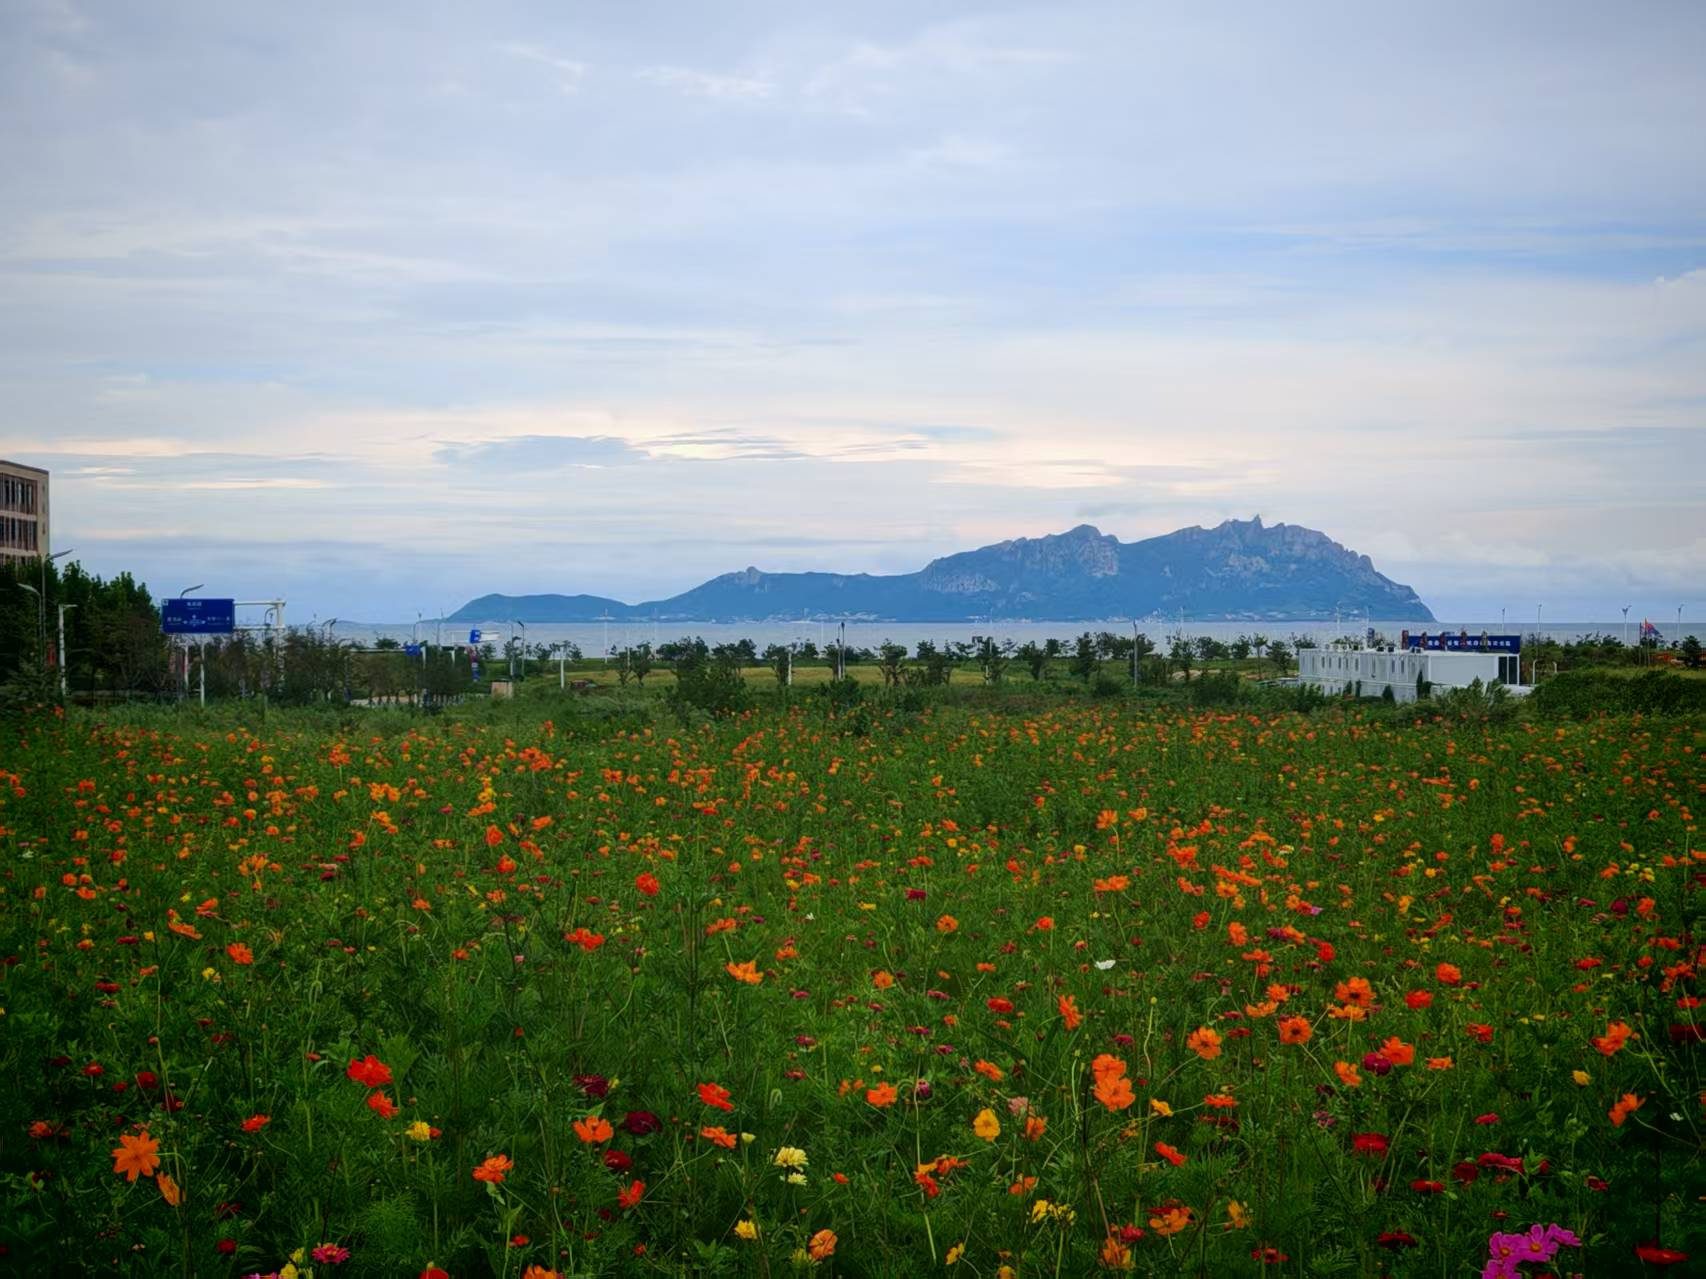
\includegraphics[width=0.6\textwidth]{images/face.jpg}
    \end{figure}
    
    \Large  
    \vspace{3cm} 
 
    \begin{tabular}{ll} 
        \textbf{主题:}& \\
        \cline{2-2} 
        \textbf{学号:} & 24020007088 \\ 
       \cline{2-2} 
        \textbf{姓名:} & 马一诺 \\  
        \cline{2-2} 
        \textbf{专业:} & 计算机科学与技术 \\  
       \cline{2-2} 
    \end{tabular}  
    \vspace{2cm}  
 
    \Large 日期: \today  
    
\end{titlepage}  

\pagenumbering{roman}
\tableofcontents


\newpage
\pagenumbering{arabic}
\section{实验目的}  

\section{实验内容及步骤}

\subsection{实验主要内容}
\subsection{实验具体步骤}
\subsection{练习记录}
\section{实例}
\subsection{实例一}
\subsection{实例二}
\subsection{实例三}
\subsection{实例四}
\subsection{实例五}
\subsection{实例六}
\subsection{实例七}
\subsection{实例八}
\subsection{实例九}
\subsection{实例十}
\subsection{实例十一}
\subsection{实例十二}
\subsection{实例十三}
\subsection{实例十四}
\subsection{实例十五}
\subsection{实例十六}
\subsection{实例十七}
\subsection{实例十八}
\subsection{实例十九}
\subsection{实例二十}
\section{实验结果}
\section{解题感悟}
\end{document}